%!TEX root = causalityRetweetPropensity.tex

\section{Discovering Causal Structure}
\subsection{Motivation}
Our goal is to identify the factors that cause or influence retweet propensity. The variables that we consider in this work are friends count, status count, followers count, klout score and sentiment. As a first step, we need to identify if there is any causal structure involving  these variables and retweets. We use the PC algorithm described in the next section. 
\subsection{Dataset}
For computational feasibility, we consider a subset of the dataset described in the previous section. We randomly sample about 1 million tweets are used for determining the causal graph structure. As mentioned above, we only look at factors friends count, status count, followers count and klout score, associated with users, and sentiment, associated with the tweet itself.
\subsection{The PC Algorithm}
Given a dataset over a set of observed random variables, and a conditional independence test, the PC(Peter Spirtes, Clark Glymour) algorithm builds a causal graph over these set of variables. The PC algorithm is based on two assumptions: \textit{Causal Markov Property} and \textit{Causal Faithfulness}. In our work, we ensure causal sufficiency by assuming that all the factors the variables involved are observed, and there are no hidden factors influencing retweets.  The PC algorithm builds the causal graph structure in two main steps. In the first step, from the data, it learns a skeleton graph, i.e., a graph with only undirected edges. As a second step, it orients the undirected edges to form a markov equivalence class of DAGs. \\
Consider a graph consisting of variables X, Y and a set of variables Z. The PC algorithm is based on the fact that, if there is no edge between variables X and Y, then there is a set of vertices Z either connected to  X or Y such that X is independent of Y, conditioned on Z, or Z d-separates  X and Y. \\

We use the R package \textit{pcalg}, that contains the implementation for PC algorithm for estimating the causal structure. We use a gaussian test for conditional independence, also built into pcalg. 

\subsection{Findings}
Figure \ref{pcoutput} shows the output of the PC algorithm. Interstingly, we see that all the factors, i.e., sentiment, followers count, status count, friends count and retweets, influence the klout score, and this could be explained by the fact that klout score is calculated based on the popularity of the user(followers, friends, status). The graph also finds that followers count influences retweets, friends count and status counts. Sentiment of a tweet also seems to influence retweet, though we will not be exploring this further in this work. The PC algorithm does not find the direction of influence between status counts and retweets. Overall, from the graph, we find an interesting interaction between followers count, status count, friends count and retweets. We explore this in more detail and attempt to find the magnitude of the influence of these factors on retweets in the next section. 
\begin{center}
\begin{figure}
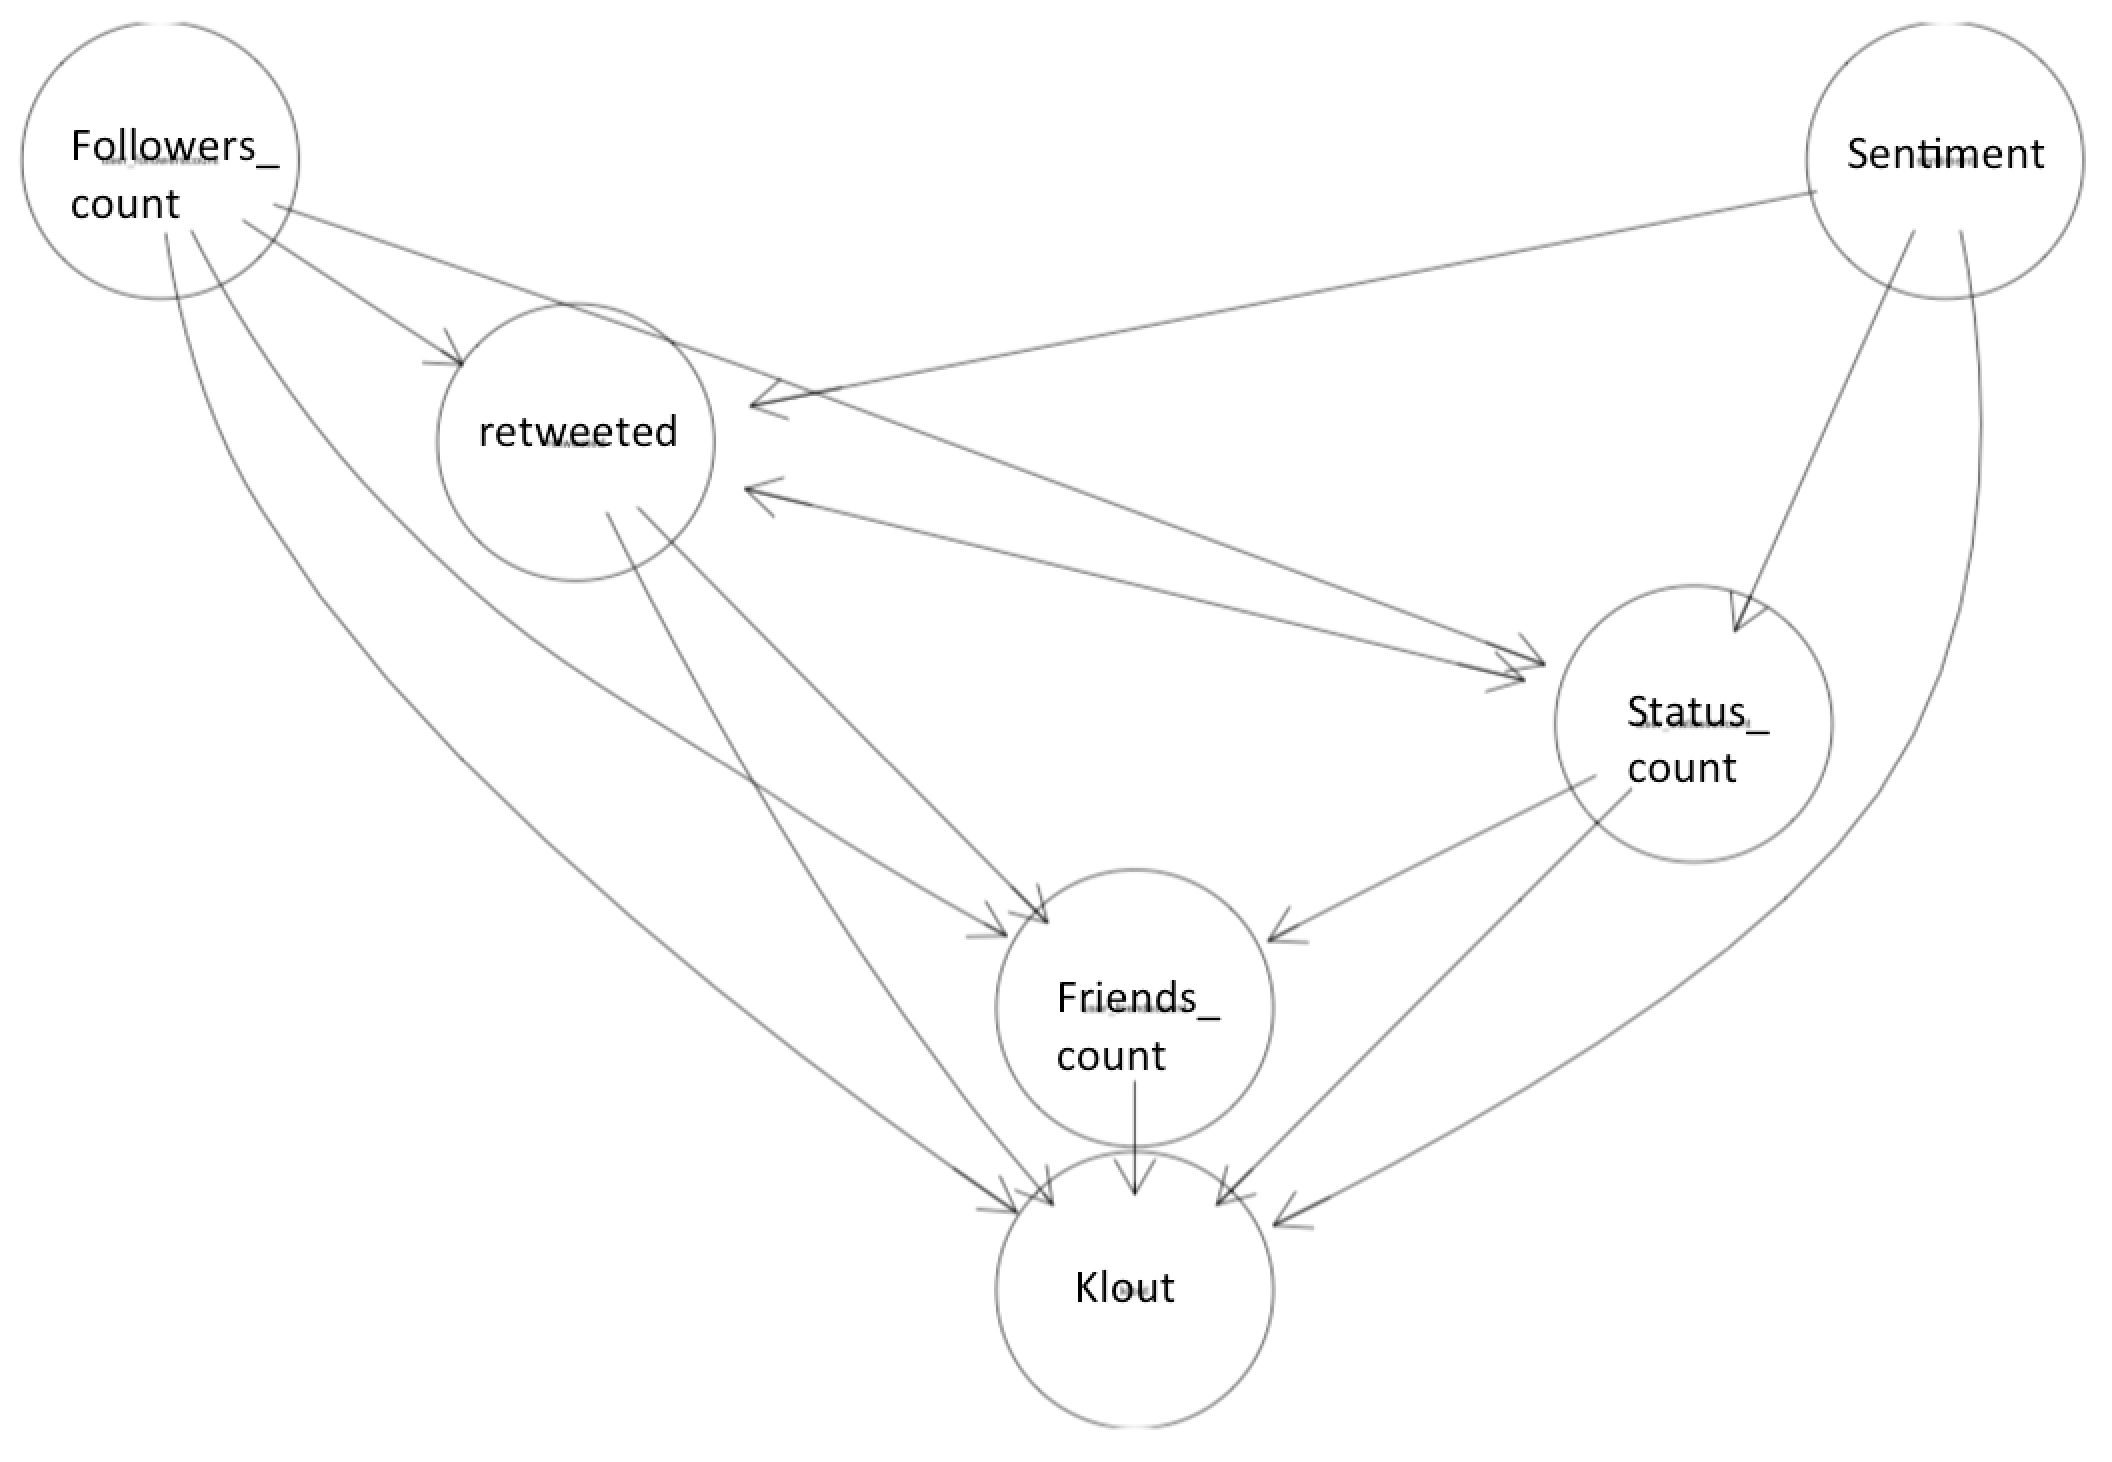
\includegraphics[scale=0.2]{pc}
\caption{Output from the PC algorithm}
\label{pcoutput}
\end{figure}
\end{center}

